\newpage
\section{Bộ dữ liệu hoa Iris}

\subsection{Tải dữ liệu và tổng quan về dữ liệu} 
\paragraph{}{\textbf{Bộ dữ liệu hoa Iris} hay bộ dữ liệu Iris của Fisher là một bộ dữ liệu đa biến nổi tiếng và được nhà thống kê và nhà sinh vật học người Anh Ronald Fisher sử dụng trong bài báo năm 1936 của ông: "The use of multiple measurements in taxonomic problems". \cite{fisher1936use}}
\paragraph{}{Bộ dữ liệu được cung cấp bởi thư viện scikit-learn.}
\begin{itemize}
    \item \textbf{150 dòng}: thông tin về 150 mẫu hoa Iris, thuộc 3 loại: Setosa, Versicolour và Virginica.
    \item \textbf{5 cột}: thông tin về kích thước hoa Iris và loại hoa, trong đó:
    \begin{itemize}
        \item \texttt{Sepal Length}: độ dài đài hoa
        \item \texttt{Sepal Width}: độ rộng đài hoa
        \item \texttt{Petal Length}: độ dài cánh hoa
        \item \texttt{Petal Width}: độ rộng cánh hoa
        \item \texttt{Target}: loại hoa (mã hóa dưới dạng 0, 1, 2)
    \end{itemize}
\end{itemize}

\begin{figure}[H]
    \centering
    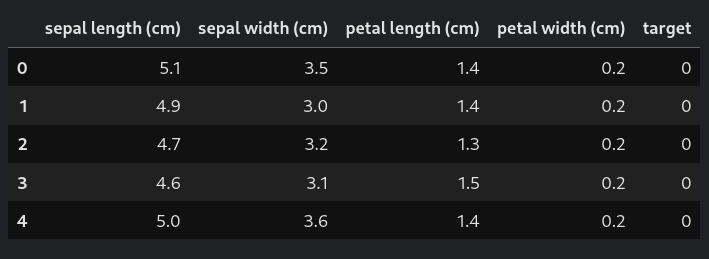
\includegraphics[width=0.8\linewidth]{img/iris_head.png}
    \caption{Các dòng đầu tiên trong bộ dữ liệu Iris}
    \label{fig:iris_head}
\end{figure}

\subsection{Phân tích và dự đoán loại hoa Iris}
\paragraph{}{Sau khi dùng chuẩn hóa \textbf{Z-score} và phân tích thành phần chính (\textbf{PCA}) trên bộ dữ liệu Iris, chúng ta thu được:}
\begin{itemize}
    \item \textbf{EVR} (Explained variance ratio) được nắm giữ bởi thành phần chính thứ nhất (PC1) và thành phần chính thứ hai (PC2) lần lượt là \texttt{0.97343527}  và \texttt{0.01707156}.
    \item \textbf{CEVR} (Cumulative explained variance ratio) của PC1 và PC2 là \texttt{0.990506835254475}.
\end{itemize}

\paragraph{}{Điều này thể hiện chỉ với hai thành phần chính đầu tiên, 99\% tỉ lệ phương sai của dữ liệu được nắm giữ bởi PC1 và PC2.}

\paragraph{}{Tiếp theo, ta áp dụng thuật toán k-means với k = 3 và thu được kết quả sau:}

\begin{figure}[H]
    \centering
    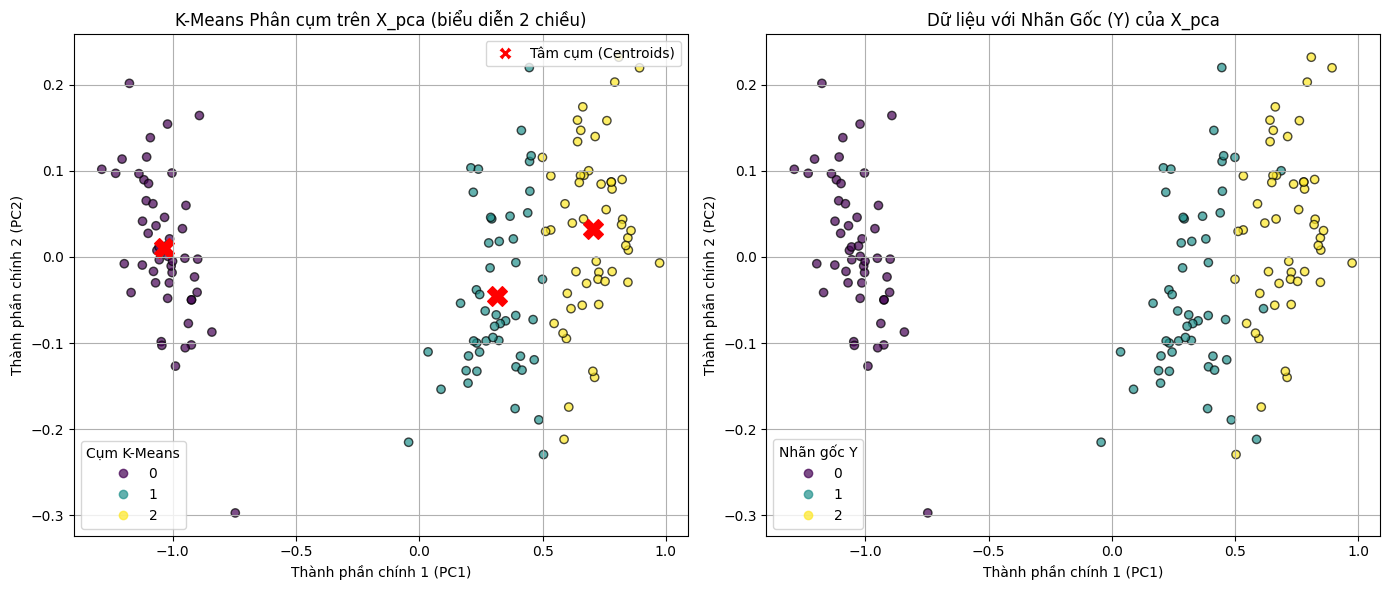
\includegraphics[width=1\linewidth]{img/iris_plot.png}
    \caption{Kết quả phân cụm trên bộ dữ liệu Iris}
    \label{fig:iris_plot}
\end{figure}

\begin{itemize}
    \item Kết quả phân cụm chính xác tới \textbf{96\%} sau khi nối nhãn với cụm phù hợp (bằng thuật toán Hungary).
    \item Ba cụm điểm dữ liệu được phân biệt rõ ràng trên mặt phẳng 2 chiều và có thể nhận biết bằng mắt thường.
\end{itemize}

\pagebreak